% Methodology: reproduction of OTPWR (Luo et al., Machines 2024)
% Needs in main.tex: amsmath, amssymb, array, booktabs, tikz (arrows.meta, positioning), pgfplots

The chosen article introduces OTPWR, a planner that gives a differential-drive mobile robot a short, collision-free and dynamically feasible trajectory. We follow its three phases and reproduce them numerically. Section~\ref{sec:flatness} uses differential flatness to reduce the planning to the plane $(x,y)$. Section~\ref{sec:astar} uses an A* search with a diagonal-distance heuristic to find the shortest collision-free sequence of grid waypoints. Section~\ref{sec:qp} joins these waypoints with piecewise polynomials whose coefficients come from a convex quadratic program (QP). Only the problem in Section~\ref{sec:qp} is a convex optimization problem; Sections~\ref{sec:flatness} and~\ref{sec:astar} provide its inputs, namely the planning variables $(x,y)$ and the waypoints.

\begin{center}
\resizebox{0.68\linewidth}{!}{%
\definecolor{stepnavy}{RGB}{31,58,95}
\definecolor{stepaccent}{RGB}{214,104,26}
\begin{tikzpicture}[
  every node/.append style={execute at begin node={\hyphenpenalty=10000\linespread{1}\selectfont}},
  card/.style={draw=gray!40, line width=0.7pt, rounded corners=4pt, fill=white,
               inner xsep=7pt, inner ysep=8pt},
  core/.style={card, draw=stepaccent, line width=1.4pt, fill=stepaccent!7},
  num/.style={circle, fill=#1, text=white, font=\bfseries\small,
              minimum size=6mm, inner sep=0pt},
  flow/.style={-{Stealth[length=2.5mm,width=1.8mm]}, line width=0.9pt, gray!60}
]
% ----- row 1 -----
\node[card] (s1) {\parbox[t][2.3cm][t]{5.2cm}{\raggedright
  {\bfseries Simplify the robot\par}\vspace{3pt}
  {\small We only follow where the robot is, $(x,y)$. Its heading and speeds can be worked out from that later, so we plan in 2D.\par}}};
\node[card, right=0.9cm of s1] (s2) {\parbox[t][2.3cm][t]{5.2cm}{\raggedright
  {\bfseries Build the map\par}\vspace{3pt}
  {\small We split the $10\times10$~m area into 1~m squares and mark each square as free or blocked.\par}}};
\node[card, right=0.9cm of s2] (s3) {\parbox[t][2.3cm][t]{5.2cm}{\raggedright
  {\bfseries Find the shortest path\par}\vspace{3pt}
  {\small A* search with the diagonal distance gives the shortest route around the obstacles, as a list of waypoints.\par}}};
% ----- row 2 -----
\node[card, below=0.7cm of s1] (s4) {\parbox[t][2.3cm][t]{5.2cm}{\raggedright
  {\bfseries Assign travel times\par}\vspace{3pt}
  {\small Each piece of the path gets a travel time, assuming the robot moves at about 0.2~m/s on average.\par}}};
\node[core, right=0.9cm of s4] (s5) {\parbox[t][2.3cm][t]{5.2cm}{\raggedright
  {\bfseries Smooth the trajectory\par}\vspace{3pt}
  {\small A convex QP draws smooth curves through the waypoints and keeps the speed and acceleration within their limits.\par}}};
\node[card, right=0.9cm of s5] (s6) {\parbox[t][2.3cm][t]{5.2cm}{\raggedright
  {\bfseries Check the results\par}\vspace{3pt}
  {\small From the curves we get the speed and turning commands, then compare our numbers with the paper.\par}}};
% ----- step numbers -----
\foreach \i in {1,2,3,4,6} \node[num=stepnavy] at (s\i.north west) {\i};
\node[num=stepaccent] at (s5.north west) {5};
\node[fill=stepaccent, text=white, font=\bfseries\scriptsize, rounded corners=2pt,
      inner xsep=4pt, inner ysep=2pt, anchor=south east] at ([xshift=-6pt]s5.north east) {CONVEX};
% ----- arrows -----
\draw[flow] (s1) -- (s2);
\draw[flow] (s2) -- (s3);
\draw[flow] (s3.south) -- ++(0,-0.35) -| (s4.north);
\draw[flow] (s4) -- (s5);
\draw[flow] (s5) -- (s6);
\end{tikzpicture}%
}
\end{center}

\subsection{Robot model and differential flatness}
\label{sec:flatness}
The motion state of the wheeled robot in a plane has two translational components $(x,y)$ and one rotational component \( \theta \). Therefore, its kinematic equations are as follows:
\begin{equation}
\begin{bmatrix}
    \dot{x} \\
    \dot{y} \\
    \dot{\theta}
\end{bmatrix}
=
\begin{bmatrix}
    \cos\theta & 0 \\
    \sin\theta & 0 \\
    0          & 1
\end{bmatrix}
\begin{bmatrix}
    v \\
    \omega
\end{bmatrix}.
\label{eq:robot_kinematics}
\end{equation}
This system is differentially flat, because all states $(x,y,\theta)$ and control inputs $(v,\omega)$ can be expressed as a function of $x$,$y$, and their time derivatives.
In this model,the planar coordinates are chosen as flat output $\sigma = [x,\,y]^T$.
Both heading and control inputs can be recovered from the time derivatives of theses outputs for any forward motion at nonzero speed:
\begin{equation}
\theta = \arctan\frac{\dot{y}}{\dot{x}}, \qquad
v = \sqrt{\dot{x}^2+\dot{y}^2}, \qquad
\omega = \frac{\ddot{y}\dot{x}-\dot{y}\ddot{x}}{\dot{x}^2+\dot{y}^2}.
\label{eq:flatness}
\end{equation}
Due to this change of variables, the trajectory optimization can be formulated in terms of $x(t)$ and $y(t)$, having obtained $\theta$,$v$,and $\omega$ from the resulting trajectory whenever the speed is nonzero. However, when the robot starts or ends at rest,$\theta$ and $\omega$ cannot be reconstructed and therefore, these endpoints need separate treatment.

\subsection{Waypoint generation by graph search}
\label{sec:astar}
A two-dimensional occupancy grid is formed by dividing the environment into discrete parts, where the beginning and final objective are depicted by unoccupied grid cells. Subsequently, a route through the grid is created.utilizing an eight-connected A* search method that enables taking into account horizontal, vertical,and diagonal movements between adjacent cells.The algorithm employs equation 3 to rank every node n, based on the total cost.The cost from the initial node to node n is denoted as g(n), while the leftover cost from node nto the final objective is approximated by h(n).
\begin{equation}
f(n) = g(n) + h(n), \qquad h(n) \le h^*(n),
\label{eq:astar}
\end{equation}
The inequality (admissibility) ensures that the path obtained is the shortest. Further-above, the diagonal distance estimation for an eight-connected grid, including a minor tie-breaking factor $p > 0$, is:
\begin{equation}
h(n) = D_s(d_x+d_y) + (D_d-2D_s)\min(d_x,d_y), \qquad h'(n) = (1+p)\,h(n),
\label{eq:heuristic}
\end{equation}
where $d_x$ and $d_y$ represent the distances from the cell to the goal. Additionally, this heuristic function never overstates the actual cost, since it corresponds to it. Nevertheless, the Manhattan distance $d_x+d_y$ could overstate the actual cost, which means that it is not the most direct route. This algorithm provides a sequenced list of waypoints
$\mathbf{w}_0,\ldots,\mathbf{w}_m \in \mathbb{R}^2$, with $\mathbf{w}_0$ and $\mathbf{w}_m$ representing the location of the objective starting point and ending. Ultimately, a segment of the trajectory is determined by two successive waypoints. This phase involves combinations and is excluded from the convex program.

\subsection{Trajectory optimization problem}
\label{sec:qp}
Each flat output ($x$ or $y$) is described by a polynomial in time:
\begin{equation}
f(t) = p_0 + p_1 t + p_2 t^2 + \cdots + p_n t^n, \qquad t\in[0,T].
\label{eq:poly}
\end{equation}
With $m+1$ waypoints from the A* search, $m$ polynomial segments are joined end to end:
\begin{equation}
f_i(t) =
\begin{cases}
\sum\limits_{j=0}^{n} p_{1j}\, t^{j}, & T_0 \le t \le T_1,\\[4pt]
\sum\limits_{j=0}^{n} p_{2j}\, t^{j}, & T_1 \le t \le T_2,\\[2pt]
\qquad\vdots & \qquad\vdots\\[2pt]
\sum\limits_{j=0}^{n} p_{mj}\, t^{j}, & T_{m-1} \le t \le T_m,
\end{cases}
\label{eq:piecewise}
\end{equation}
where $p_{mj}$ is the $j$-th coefficient of segment $m$ and $T_1,\dots,T_m$ are the segment times.

\paragraph{Objective.}
The cost of segment $j$ is the integral of its squared $k$-th derivative:
\begin{equation}
J_j(T) = \int_{T_{j-1}}^{T_j} \big(f^{(k)}\big)^2\, dt.
\label{eq:segint}
\end{equation}
All derivatives depend linearly on the coefficients, so this integral is a quadratic form.
\begin{equation}
J_j(T) = p_j^T H_j\, p_j,
\label{eq:quad}
\end{equation}
where $p_j = [p_0, p_1, \dots, p_n]^T$ and $H_j$ depends only on the segment times. Adding all $m$ segments gives the objective
\begin{equation}
J_{\text{total}} =
\begin{bmatrix} p_1\\ \vdots\\ p_m \end{bmatrix}^T
\begin{bmatrix} H_1 & & \\ & \ddots & \\ & & H_m \end{bmatrix}
\begin{bmatrix} p_1\\ \vdots\\ p_m \end{bmatrix}.
\label{eq:objective}
\end{equation}

\paragraph{Constraints.}
Three sets of linear restrictions operate on the coefficients. The terminal restrictions determine the slopes of every section at both boundary points.
\begin{equation}
f_j^{(k)}(T_{j-1}) = d^{(k)}_{j,1}, \qquad f_j^{(k)}(T_j) = d^{(k)}_{j,2},
\label{eq:endpoint}
\end{equation}
which, for all segments, give
\begin{equation}
\begin{bmatrix} A_1\\ \vdots\\ A_m \end{bmatrix}
\begin{bmatrix} p_1\\ \vdots\\ p_m \end{bmatrix}
=
\begin{bmatrix} d_1^{(k)}\\ \vdots\\ d_m^{(k)} \end{bmatrix}.
\label{eq:Aeq}
\end{equation}
Continuity requirements ensure derivatives of adjacent segments match at the point where they gather,
\begin{equation}
f_j^{(k)}(T_{j,2}) = f_{j+1}^{(k)}(T_{j,1}),
\label{eq:cont}
\end{equation}
which give
\begin{equation}
\begin{bmatrix} B_1\\ \vdots\\ B_m \end{bmatrix}
\begin{bmatrix} p_1\\ \vdots\\ p_m \end{bmatrix}
=
\begin{bmatrix} 0\\ \vdots\\ 0 \end{bmatrix}.
\label{eq:Beq}
\end{equation}
Kinematic limits keep the velocity and acceleration within a minimum and maximum permitted range tied,
\begin{equation}
-d^{k}_{j,\mathrm{lb}} \le f_j^{(k)}(T_{j,2}) \le d^{k}_{j,\mathrm{ub}},
\label{eq:bound}
\end{equation}
which give
\begin{equation}
\begin{bmatrix} C_1\\ \vdots\\ C_m \end{bmatrix}
\begin{bmatrix} p_1\\ \vdots\\ p_m \end{bmatrix}
\le
\begin{bmatrix} -d^{(k)}_{1,\mathrm{lb}}\\ \vdots\\ d^{(k)}_{m,\mathrm{ub}} \end{bmatrix}.
\label{eq:Cineq}
\end{equation}
We employ fifth-degree polynomials ($n=5$) and minimize the snap ($k=4$). Endpoint conditions for \(k=0\) ensure that the path traverses every waypoint (C1), while those for \(k=1,2\) impose zero velocity and acceleration at both the initial point and final destination (C2). Continuity of velocity and acceleration (k=1,2) is enforced at each of the m-1 junctions (C3), where the respective bounds are ±0.5 m/s and ±0.2 m/s² (C4).

Putting the objective and the constraints together gives the QP
\begin{equation}
\begin{aligned}
\min \quad & J_{\text{total}}\\
\text{s.t.} \quad &
\begin{cases}
A p = d^{(k)},\\
B p = 0,\\
C p \le d^{(k)}_{\mathrm{lb},\mathrm{ub}}.
\end{cases}
\end{aligned}
\label{eq:qp}
\end{equation}

\subsection{Convexity analysis}
%Each term $p_j^T H_j p_j$ is the integral of a square, so it can never be negative for any $p_j$. This means $H_j\succeq 0$, and $J(p)$ is a convex quadratic. $H$ is singular because the coefficients of degree below four do not appear in the snap, so the objective is convex but not strictly convex; those coefficients are fixed by the equality constraints. All the constraints (C1)--(C4) are affine in $p$, so the feasible set is a polyhedron. A convex quadratic minimized over a polyhedron is a convex QP, so any local minimum is global and the solver returns the best coefficients for the given waypoints and segment times.
The objective for a fixed segment duration \(T_j\), is a quadratic function of the polynomial coefficients. Furthermore, for every coefficient vector \(p_j\),
\[
    p_j^\top H_j p_j
    =\int_0{T_j} \bigl(x_j^{(4)}(\tau)\bigr)^2\,d\tau \geq 0
\]
Therefore, every \(H_j\) is positive semidefinite, and  in result, the block-diagonal matrix \(H\) is also positive semidefinite. Thus, the objective \(J(p)=p^\top Hp\) is convex. Moreover,fixing the waypoints and segment duration, the constraints (C1)--(C3) become affine equalities in \(p\), and each absolute-value bound in (C4) is equivalent to two affine inequalities in \(p\). As a result,  the feasible set is a polyhedron. Thus,the trajectory optimization is a convex quadratic program, where every local minimizer is global.

\subsection{Approximations and their implications}
%The segment times $T_j$ are fixed, because optimizing them together with $p$ would make the problem non-convex; the trajectory is therefore optimal only for the chosen times, which the article does not report. The trajectory is also tied to the A* waypoints at the cell centres. The limits in (C4) are imposed only at the junctions and on each axis separately, so the speed can exceed $v_{\max}$ inside a segment and reach $\sqrt{2}\,v_{\max}$ on a diagonal. Nothing in the QP prevents a collision between two waypoints. Finally, we write each segment in local time instead of the article's global time; this gives the same trajectories but keeps $H_j$ well conditioned.
Before solving the trajectory quadratic program, the waypoints generated by the A* algorithm and the segment durations \(T_j\) are fixed. Moreover, the endpoint constraints would contain products such as \(p_{j,i}T_j^i\) if the durations were optimized jointly with the polynomial coefficients. As a result, the joint formulation becomes generally nonconvex. Thus, the snap objective for the prescribed waypoints and durations is minimized by the resulting trajectory.
In (C4) the bounds are applied separately to each coordinate at the segment junctions. Furthermore, if both velocity components reach their limits, the planar speed at those junctions can reach \(\sqrt{2}\,v_{\max}\). No speed or acceleration guarantee can be provided by (C4) between the junctions.Moreover, the waypoint constraints allow for the intersection of obstacles with the polynomial trajectory between successive waypoints.
In this project, each polynomial is expressed in local segment time. By doing this change of variable, the set of trajectories is preserved and the numerical scaling can be improved by avoiding powers of large global time values.
Therefore, the QP results in a minimum-snap trajectory subject to the imposed constraints. To verify collision avoidance and compliance with motion limits over each full segment, checking the trajectory between junctions is required.
\subsection{Implementation and validation}
%We implement the method in MATLAB, as the article did (MATLAB R2021a), with YALMIP, and solve the QP with \texttt{quadprog} or OSQP, the solver cited in the article. We rebuild Grid Maps~1 and~2 of the article ($10\times10$~m, 1~m cells, start $(0.5,0.5)$, goal $(8.5,8.5)$) from its figures, and run Dijkstra, Euclidean, Manhattan and diagonal A* with $D_s=1$, $D_d=\sqrt{2}$ and $p=0.001$. Since the segment times are not given, we use $T_j=\lVert w_j-w_{j-1}\rVert/0.2$~m/s, which agrees with the article's Figs.~9--10, where a path of about 13~m takes about 65~s.
%For the path search, the lengths should match the article exactly (12.4853~m and 13.8995~m); search times and visited nodes depend on the computer, so we compare their ranking. For the trajectory, we check the solver status, that (C1)--(C4) hold, the peak speed and acceleration inside each segment, and the total duration.
Following the article's MATLAB simulation setup, we will reconstruct Grid Maps 1 and 2 from Figs.~7 and~8 of the article using Python. Each map is a $10 \times 10\, \mathrm{m}$ with $1\,\mathrm{m}$ cells grid, with a start position at $(0.5,0.5)\,\mathrm{m}$ and end goal position at $(8.5,8.5)\,\mathrm{m}$. For each map, a Dijkstra's algorithm and A* with Eucledian, Manhattan, and diagonal heuristics will be ran. Moreover, the cost of axial and diagonal moves are $D_s=1$ and $D_d=\sqrt{2}$ respectively. The heuristic adjustment in Eq.~(2) with $p=0.001$ is used for the diagonal A$^{*}$.
\begin{figure}[!htbp]
    \centering
    \begin{minipage}[t]{0.48\linewidth}
    \centering
    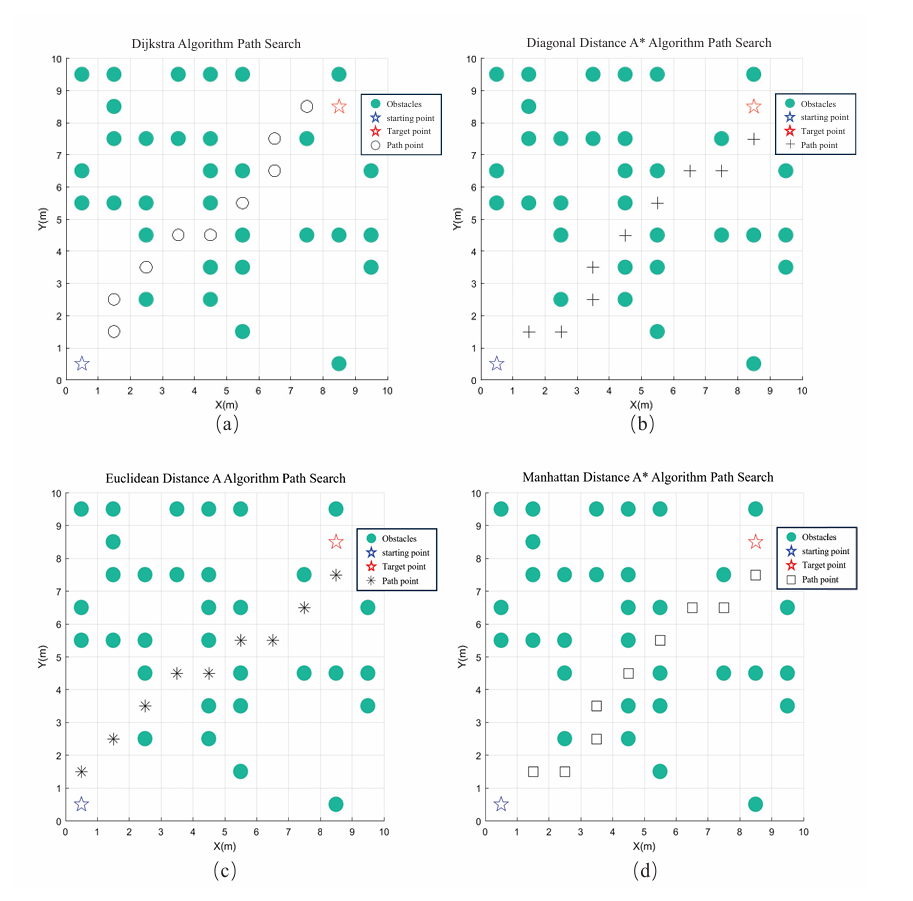
\includegraphics[height=3.8cm,width=\linewidth,keepaspectratio]{karem/article_fig7.png}
    \caption{Path-search results on Grid Map 1 from Fig.~7
    of Luo et al.~\cite{luo2024otpwr}.}
    \label{fig:article_grid_map_1}
    \end{minipage}\hfill
    \begin{minipage}[t]{0.48\linewidth}
    \centering
    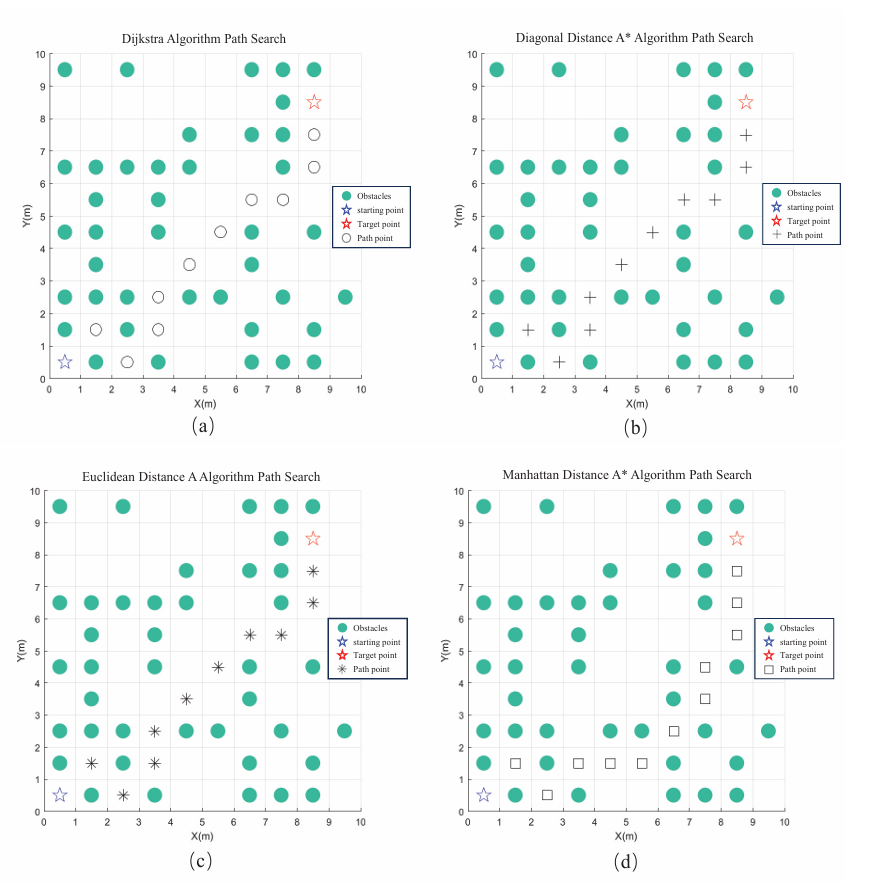
\includegraphics[height=3.8cm,width=\linewidth,keepaspectratio]{karem/article_fig8.png}
    \caption{Path-search results on Grid Map 2 from Fig.~8
    of Luo et al.~\cite{luo2024otpwr}.}
    \label{fig:article_grid_map_2}
    \end{minipage}
\end{figure}

The computed path length will be compared with the values reported in Tables~1 and~2 of the article. For all four methods, the reference path length on Grid Map~1 is $12.4853\,\mathrm{m}$. However, with respect to Grid Map~2, the reference path length is $13.8895\,\mathrm{m}$ for Dijkstra's algorithm, Eucledian A$^{*}$, and diagonal A$^{*}$, and $14.4853\,\mathrm{m}$ for Manhattan A$^{*}$. Moreover, a comparison between the number of expanded nodes and the median search time over repeated runs will be done. Noting that node counts can vary with the search implementation, the runtime also depends on the computing environment. 

The waypoints generated by the diagonal A$^{*}$ are used for trajectory generation. Since the individual segment durations are not reported in the article, a duration proportional to the distance between consecutive waypoints will be assigned.
\begin{equation}
    T_j=\frac{\lVert w_j-w_{j-1}\rVert_2}{v_{\mathrm{ref}}},\qquad v_{\mathrm{ref}}=0.2\,\mathrm{m/s}.
    \label{eq:segment_duration}
    \end{equation}
$v_{\mathrm{ref}}$ is chosen based on the approximate distance and time scales in Figs.~9 and~10 of the article. While holding the segment durations fixed, the minimum-snap QP will be formulated in CVXPY and solved with OSQP.
\begin{figure}[!htbp]
    \centering
    \begin{minipage}[t]{0.42\linewidth}
    \centering
    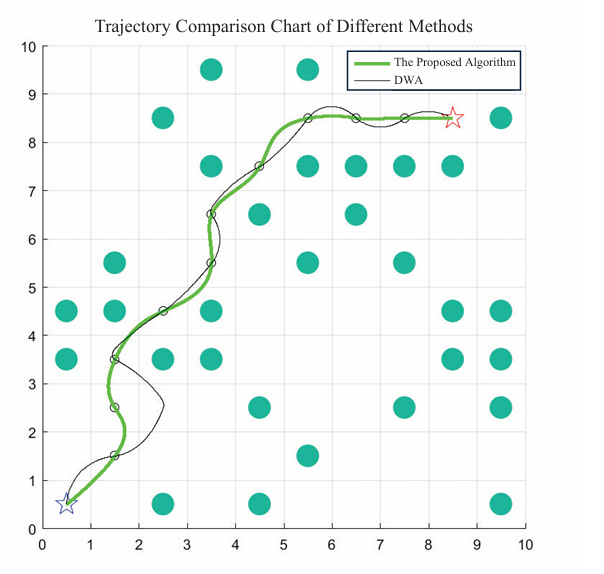
\includegraphics[height=3.7cm,width=\linewidth,keepaspectratio]{karem/article_fig9.png}
    \caption{Comparison of trajectories generated by OTPWR and DWA from Fig.~9 of Luo et al.~\cite{luo2024otpwr}.}
    \label{fig:article_trajectory_comparison}
    \end{minipage}\hfill
    \begin{minipage}[t]{0.54\linewidth}
    \centering
    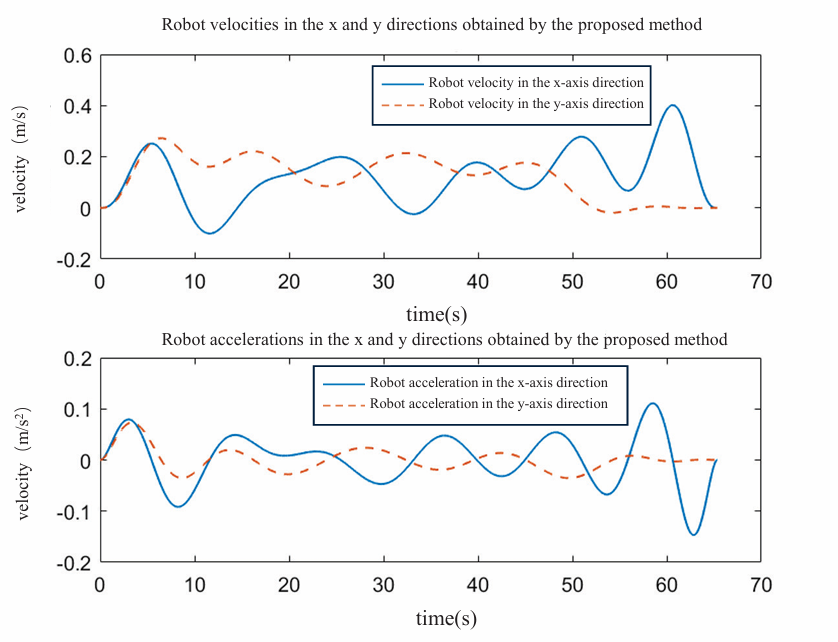
\includegraphics[height=3.7cm,width=\linewidth,keepaspectratio]{karem/article_fig10.png}
    \caption{Velocity and acceleration components for the OTPWR trajectory from Fig.~10 of Luo et al.~\cite{luo2024otpwr}.}
    \label{fig:article_motion_profiles}
    \end{minipage}
\end{figure}

Finally, the solver status, integrated snapm residuals for constraints (C1)--(C4), and the prescribed total duration $\sum_j T_j$ will be reported for each trajectory. The trajectory between junctions will be evaluated to estimate the peak planar speed and acceleration, assess the componentwise velocity and acceleration bounds, and check for intersection with occupied cells.

\subsection{Planned extensions}
%All four extensions keep the problem convex. E1 replaces the box limits with a true speed limit $\lVert[\dot{x}_j(\tau_s),\,\dot{y}_j(\tau_s)]\rVert_2\le v_{\max}$ at sample times $\tau_s$, which turns the QP into an SOCP. E2 imposes the limits at several points inside each segment. E3 keeps sampled positions inside obstacle-free rectangles (safe corridors). E4 compares minimum jerk with minimum snap and tests how sensitive the results are to the segment times and limits.
The article's ~\cite{luo2024otpwr} problem formulation enforces motion limits at segment joints, which may cause violations between junctions. In the same manner, obstacle free waypoints alone do not ensure that the trajectory connecting them avoids obstacles. Therefore, based on the article's minimum-snap formulation,  four extensions to the trajectory optimization problem are proposed. Moreover, for each proposed formulation, the segment durations, sample times, and any corridor assignments are fixed before solving, yielding a convex optimization problem.

\begin{enumerate}
    \item [\textbf{E1.}] \textbf{Planar speed limit.}
    At the segment junctions, the componentwise velocity bounds are replaced with a bound on the magnitude of the planar velocity:
    \[
    \left\lVert
    \begin{bmatrix}
        \dot{x}_j(\tau_s)\\
        \dot{y}_j(\tau_s)
        \end{bmatrix}
        \right\rVert_2\leq v_{\max}
    \]
    The velocity components are affine in the polynomial coefficients at each prescribed time $\tau_s$, therefore, this is a second order cone constraint.

    \item[\textbf{E2.}] \textbf{Bounds within each segment.}
    To reduce violations between junctions, the velocity and acceleration limits are enforced at additional sample times within each segment. When tested separattely from E1, this extension uses componentwise bounds. Thus the problem remains a QP.

    \item[\textbf{E3.}] \textbf{Obstacle-free corridors.}
    Before solving, an obstacle-free rectangle is assigned to each segment, and the sampled positions along that segment are constrained so that they lie inside that rectangle. These constraints are linear in the polynomial coefficients, collisions between sample times are checked separately.

    \item[\textbf{E4.}] \textbf{Objective comparison and sensitivity.}
    Using the same waypoints, segment durations, and constraints, the minimum-jerk trajectory is compared with the minimum-snap one. Then, to assess how the prescribed segment durations and motion limits affect feasibility and resulting trajectories, the optimizations are repeated across varying combinations of these parameters.
\end{enumerate}